\documentclass[14pt]{matmex-diploma-custom}

\usepackage{syntax}
\usepackage{listings}
\usepackage{caption}
\usepackage{stfloats}


\lstdefinelanguage{Pseudocode}
{
  morekeywords={input, output, return, datatype, function, in, if, else, foreach, while, begin, end},
  morecomment=[l]{--},
  morecomment=[s]{/*}{*/},
  morestring=[b]"
}

\lstdefinestyle{Pseudo} {
    language        = Pseudocode,
    basicstyle      = \footnotesize\ttfamily,
    identifierstyle = \color{black},
    commentstyle    = \color{red},
    keywordstyle    = \color{blue},
    stringstyle     = \color{red},
    extendedchars   = true,
    tabsize         = 4,
    showspaces      = false,
    showstringspaces = false,
    breakautoindent = true,
    flexiblecolumns = true,
    keepspaces      = true,
    stepnumber      = 0,
    xleftmargin     = 0pt
}
\lstset{
    style=Pseudo,
    breaklines=false,
    frame=single
}


% Python language

\lstdefinelanguage{Python}
{
  morekeywords={if , for, in},
  morecomment=[l]{#},
  morestring=[b]"
}

\lstdefinestyle{Python} {
    language=Python,
    basicstyle=\ttm,
    commentstyle= \color{red},
    otherkeywords={self},             % Add keywords here
    keywordstyle=\ttb\color{deepblue},
    % emph={MyClass,__init__},          % Custom highlighting
    emphstyle=\ttb\color{deepred},    % Custom highlighting style
    stringstyle=\color{deepgreen},
    frame=tb,                         % Any extra options here
    showstringspaces=false            % 
}



\begin{document}

\filltitle{ru}{
    chair              = {Кафедра технологии программирования},
    title              = {Предсказание исполнителя задания в системе электронного документооборота},
    % Здесь указывается тип работы. Возможные значения:
    %   coursework - Курсовая работа
    %   diploma - Диплом специалиста
    %   master - Диплом магистра
    %   bachelor - Диплом бакалавра
    type               = {coursework},
    position           = {студента},
    group              = 307,
    author             = {Буланина Екатерина Дмитриевна},
    supervisorPosition = {к.\,ф.-м.\,н., доцент},
    supervisor         = {Добрынин В.\,Ю.},
%    reviewerPosition   = {},
%    reviewer           = {},
    chairHeadPosition  = {к.\,т.\,н., доцент},
    chairHead          = {Блеканов И.\,С.},
%   university         = {Санкт-Петербургский Государственный Университет},
%   faculty            = {Факультет прикладной математики - процессов управления},
%   city               = {Санкт-Петербург},
%   year               = {2018}
}
\filltitle{en}{
    chair              = {Applied Mathematics and Control Processes Faculty \\ Programming Technology Chair},
    title              = {Assignee prediction in document automation system},
    author             = {Ekaterina Bulanina},
    supervisorPosition = {},
    supervisor         = {Vladimir Dobrynin},
    chairHeadPosition  = {},
    chairHead          = {Ivan Blekanov},
}
\maketitle
\tableofcontents
% У введения нет номера главы
\section*{Введение}
Во многих компаниях, оперирующих с большим количеством документов, для автоматизации и ускорения работы используются системы электронного документооборота. Такие системы значительно уменьшают время таких операций с документами, как регистрация, рассылка, хранение или использование содержащейся в них информации.

Современные системы электронного документооборота (СЭД) при помощи компьютерной обработки и методов машинного обучения добавляют множество новых возможностей: распознавание и выгрузка текстов из отсканированных изображений, автоматическое определение типа документа и т.д.

Задача автоматического назначения исполнителя задания является интересной в контексте анализа данных, а её решение способствует расширению функционала СЭД. Исполнитель --- это сотрудник, который будет обрабатывать документ и, после выполнения над ним необходимых операций, передавать его другому сотруднику. Для компаний с большой иерархической организацией было бы очень полезно заранее знать, какую последовательность (цепочку) исполнителей пройдет созданный в системе документ.

Одной из наиболее популярных систем документооборота в России является система Docsvision~\cite{docsvision}, представляющая из себя платформу для организации и автоматизации управления в отраслях государственного сектора, банковской сферы, оборонно-промышленного комплекса и других областей.

\section{Постановка задачи}
Целью данной работы является создание инструмента для предсказания цепочки исполнения документа. Для этого были поставлены следующие задачи:
\begin{itemize}
    \item Провести анализ данных, предоставленных компанией Digital Design~\cite{digdes};
    \item Выполнить обзор существующих подходов для предсказания исполнения и выбрать подходящий;
    \item Реализовать выбранный алгоритм;
    \item Протестировать полученную реализацию.
\end{itemize}

\section{Обзор}
В качестве основного источника для изучения методов машинного обучения и анализа данных я использовала книгу К. Маннинга <<Введение в информационный поиск>>~\cite{Manning}. В этом учебнике рассматривается современный подход ко всем аспектам проектирования и внедрения систем сбора, индексирования и поиска документов, методы оценки систем и использование методов машинного обучения в наборах текстов. В частности, в этой книге описываются алгоритмы стемминга и лемматизации, которые используются в данной работе.

Основной алгоритм, использованный в решении задачи, --- алгоритм Apriori~\cite{apriori-algorithm}. Этот алгоритм реализует поиск ассоциативных правил~\cite{association-rule-first} (т.е. зависимостей между элементами) в больших наборах данных. Использование этого алгоритма для предсказания исполнителя хорошо описано в статье <<Bug Assignee Prediction Using Association Rule Mining>>~\cite{Sharma}. В ней рассматривается решение задачи предсказания разработчика, который будет работать над исправлением ошибки в проекте. Авторы статьи анализируют ассоциативные правила, найденные алгоритмом Apriori, для предсказания на примере пяти ведущих разработчиков в нескольких проектах.

Отдельного внимания требует работа Н. Чурикова~\cite{Churikov}. В этой работе рассматривается задача рекомендации исполнителя документа и методы её решения. Моя работа представляет альтернативный подход для решения этой задачи.

При реализации решения задачи я использовала язык Python и библиотеки Pandas и NumPy, для изучения которых была полезна книга В. МакКини <<Python для анализа данных>>~\cite{mckinney}.

\section{Исследование предоставленных данных}
Во время регистрации документа в системе Docsvision заполняется форма, представленная ниже. В ней вручную или автоматически заполняются параметры (атрибуты) документа: тип, автор, категория, краткое описание и т.п. После загрузки в базу DocsVision документ и его атрибуты представляют собой метаданные, хранящиеся в формате JSON. Аналогичным образом представляются в системе задания, атрибутами которых могут служить время создания, срочность и описание поручения. Задания также хранятся в формате JSON.

\begin{figure}[h]
\caption{Создание документа в системе DocsVision}
\centering
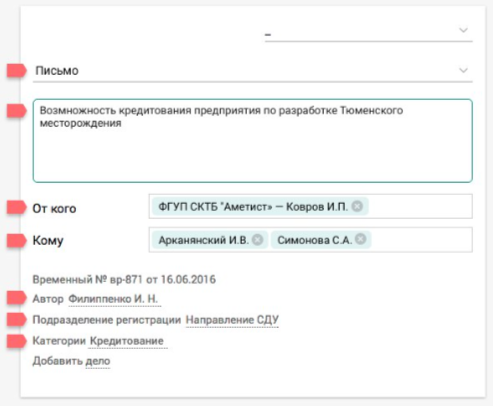
\includegraphics[width=0.4\textwidth]{images/letter.png}
\end{figure}

В полученных JSON-файлах атрибуты документа как правило представляют собой категориальные переменные или текст. Категориальные переменные задаются в виде \textit{UUID}~\cite{uuidwiki}, который является уникальным значением вида xxxxxxxx-xxxx-Mxxx-Nxxx-xxxxxxxxxxxx, где M и N задают версию идентификатора, а x является произвольной латинской буквой или цифрой. Каждому документу соответствует \textit{резолюция} --- файл, хранящий в себе последовательность заданий в порядке их создания. Каждое задание характеризуется \textit{атрибутами} и \textit{исполнителем}. Исполнители бывают двух видов: Appointed (тот, кто был назначен на задание при его создании) и Executes (тот, кто непосредственно выполнял задание). Специфика данных такова, что Appointed и Executes обычно совпадают. Поэтому в представленной реализации анализируются только те, кто был назначен на задание. Однако в общем случае данный подход можно расширить.

\section{Реализация}
Для осуществления поставленной задачи была произведена лемматизация слов, из которых состоит описание документа. Для реализации этого использовались библиотеки обработки естественного языка Natural Language Toolkit~\cite{nltk} и PyMyStem3~\cite{yandex}. Далее для каждого исполнителя с $1..k$ уровня исполнения любого документа в словарь заносится набор слов из описания документов как показано в листинге~\ref{lst:dict}.

После того, как известен набор слов, появлявшихся в описаниях документов исполнителей, можно применить поиск ассоциативных правил алгоритмом Apriori, представленный в листинге~\ref{lst:apriori}.

\begin{lstlisting}[language=Python,caption={Псевдокод создания словаря исполнителей},captionpos=t,label={lst:dict}]
people = {}
for doc in dataBase:
    assignees = doc.resolution['Executes'] # получение цепочки исполнителей документа
    for assignee in assignees:
        people[assignee] += doc.description
\end{lstlisting}

\begin{lstlisting}[caption={Псевдокод алгоритма Apriori},captionpos=t,label={lst:apriori}, mathescape=true]
$L_1 = \{large~1-item sets\}$
$k$ $=$ $2$
$\mathrm{\textbf{while}}$ $L_{k-1}$ $\neq  \{\}:$
$&\qquad C_k$ $= \{ a \cup \{b\} \mid a \in L_{k-1} \land b \not \in a \} - \{ c \mid \{ s \mid s \subseteq c \land |s| = k-1 \} \not\subset L_{k-1} \}$
$&\qquad\mathrm{\textbf{for}~transactions}~t \in T:$
$&\qquad\qquad C_t = \{ c \mid c \in C_k \land c \subseteq t \} $
$&\qquad\qquad \mathrm{\textbf{for}~candidates}~c \in C_t$
$&\qquad\qquad\qquad \mathit{count}[c] = \mathit{count}[c]+1$
$&\qquad L_k = \{ c \mid c \in C_k \land ~ \mathit{count}[c] \geq \epsilon \}$
$&\qquad k = k+1\\$
$&\mathrm{\textbf{return}}~\bigcup_k L_k$
\end{lstlisting}



\section{Эксперименты}
Полученная реализация была протестирована на данных от компании Digital Design. Данные представляли собой 131215 документов Правительства Мурманской области. Ниже в таблице представлены ассоциативные правила для нескольких исполнителей с наибольшим числом заданий. 

Support --- выраженное в процентах отношение числа документов, в которых встретились указанные термы и данный исполнитель, к общему числу рассматриваемых документов (в моем случае выборка из трех исполнителей с наибольшим числом заданий).

Confidence --- выраженное в процентах отношение числа документов, на которых был назначен указанный исполнитель, к числу документов, в которых встретились указанные термы.

\begin{table}[hb]
\centering
\caption{Ассоциативные правила для Дмитриенко}
\label{my-label}
\begin{tabular}{|l|l|l|l|}
\hline
\# & {[}terms{]} $\rightarrow$ Дмитриенко & Confidence & Support \\ \hline
1 & \begin{tabular}[c]{@{}l@{}}{[}'губернатор', 'данные', 'оперативный',\\  'перечень', 'поручение'{]}\end{tabular} & 1.9269 & 71.2215 \\ \hline
2 & {[}'перечень', 'поручение', 'совещание'{]} & 2.0614 & 70.229 \\ \hline
3 & \begin{tabular}[c]{@{}l@{}}{[}'данные', 'оперативный', 'перечень',\\  'совещание'{]}\end{tabular} & 1.9606 & 70.994 \\ \hline
4 & {[}'контроль', 'поручение', 'снятие'{]} & 1.2043 & 65.7492 \\ \hline
5 & \begin{tabular}[c]{@{}l@{}}{[}'2011', 'губернатор', 'данные', 'оперативный',\\  'перечень', 'поручение', 'совещание'{]}\end{tabular} & 1.3836 & 65.1715 \\ \hline
6 & {[}'контроль', 'перечень', 'поручение', 'снятие'{]} & 1.1091 & 68.9895 \\ \hline
\end{tabular}
\bigskip
\centering
\caption{Ассоциативные правила для Портная}
\label{my-label}
\begin{tabular}{|l|l|l|l|}
\hline
\# & {[}terms{]} $\rightarrow$ Портная & Confidence & Support \\ \hline
1 & {[}'2011', 'перечень', 'поручение'{]} & 1.0979 & 37.3333 \\ \hline
2 & {[}'исполнение', 'продление', 'срок'{]} & 1.1987 & 69.2556 \\ \hline
3 & {[}'направлять', 'рф'{]} & 1.0123 & 99.13 \\ \hline
4 & \begin{tabular}[c]{@{}l@{}}{[}'данные', 'оперативный', 'перечень',\\  'поручение', 'совещание'{]}\end{tabular} & 1.2697 & 98.12 \\ \hline
\end{tabular}
\end{table}

\section*{Заключение}
В ходе выполнения работы были получены следующие результаты:
\begin{itemize}
    \item Исследованы данные, предоставленные компанией Digital Design;
    \item Проведен обзор предметной области и изучены существующие подходы к решению задачи;
    \item Реализован алгоритм Apriori;
    \item Полученная реализация протестирована на предоставленных данных.
\end{itemize}

\setmonofont[Mapping=tex-text]{CMU Typewriter Text}
\bibliographystyle{ugost2008ls}
\bibliography{diploma.bib}
\end{document}
